\documentclass[10pt]{article}
\setlength{\topmargin}{-0.5in}
\setlength{\oddsidemargin}{0.0in}
\setlength{\evensidemargin}{0.0in}
\setlength{\textheight}{9in}
\setlength{\textwidth}{6.5in}

\renewcommand{\thepage}{p. \arabic{page} \quad -- \quad 03/12/2004}

\newcommand{\bing}{{\bf BING!} }
\newcommand{\goto}[1]{\bing \vskip 12pt \section*{{\em{#1}}}}
\usepackage{graphicx}
\begin{document}

\begin{center}

MIT Science Fiction Society 

84 Massachusetts Avenue

Cambridge, MA 02139

\vspace{12pt}

MITSFS Meeting Minutes 

Friday, March 12, 2004

\end{center}
 
\vspace{18pt}

\setlength{\parskip}{6pt}

\noindent
Pre-meeting quote: ``The UA election regulations don't actually
prevent you from lying to your constituencies.  They regulate poster
violations.''-ARM

MITSFS meeting called to order, 1700 SST, Ed Keyes, President and
Skinner, presiding; Kat Allen,  Onseck, recording.

Minutes read.

BTS corrects that Alan Moore wrote League of Extraordinary Gentlemen
*before* the script proposal

Enorse the counterconspiracy theory of history: that the effect
conspiracy theories have had on history is greater than any possible 
Passes 12-2-2+Spehn

Motion to have the Onseck record the minutes in comic book form
Passes 11-0-0+Spehn
 
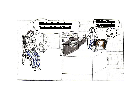
\includegraphics[height = 3in]{panel.2004-03-12.01.eps}

\subsection*{TZ}
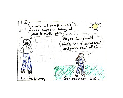
\includegraphics[height = 3in]{panel.2004-03-12.02.eps}

\subsection*{MobComm}
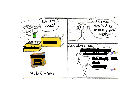
\includegraphics[height = 3in]{panel.2004-03-12.03.eps}

\subsection*{LHE}
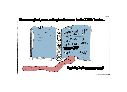
\includegraphics[height = 3in]{panel.2004-03-12.04.eps}

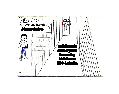
\includegraphics[height = 3in]{panel.2004-03-12.05.eps}

\subsection*{We could send the books by interdepartmental mail and
  increase the Library's size...}
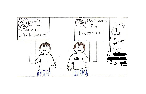
\includegraphics[height = 3in]{panel.2004-03-12.06.eps}

\subsection*{ARM reveals his plan}
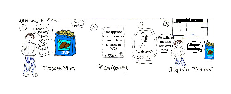
\includegraphics[width = 5in]{panel.2004-03-12.07.eps}

\subsection*{New Guinea Report}
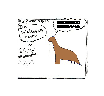
\includegraphics[height = 3in]{panel.2004-03-12.08.eps}

\subsection*{This makes no sense to me, either}
\includegraphics[height = 3in]{panel.2004-03-12.09.eps}

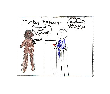
\includegraphics[height = 3in]{panel.2004-03-12.10.eps}

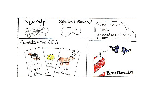
\includegraphics[height = 3in]{panel.2004-03-12.11.eps}

\subsection*{Miller Motion}
\includegraphics[width = 5in]{panel.2004-03-12.12.eps}


Motion: End the meeting without a Miller or Banana Motion\\
Passes 13-0-1+Spehn

\noindent
Meeting adjourned, 1730 SST.

\vspace{18pt}

\centerline{Respectfully submitted,}
\centerline{Kat Allen,  Onseck}

\end{document}
